\lab{ARMA Models}{ARMA Models}
\label{lab:arma}
\objective{Fit and forecast ARMA models.}

An $\text{ARMA}(p,q)$ model is a covariance-stationary discrete stochastic
process $\{z_t\}$ that satisfies
\begin{align}
    \label{eq:arma:def}
    z_t - \mu = \left(\sum_{i=1}^p \phi_{i}(z_{t - i} - \mu)\right) + a_t +
    \left(\sum_{j=1}^{q} \theta_{j}a_{t-j} \right)
\end{align}
where $\mu = E[z_t]$ and $a_t$ are identically Gaussian distributed with
variance $\sigma_a^2$. We note that the assumption that $\{z_t\}$ is
covariance-stationary is eqivalent to the condition that the roots of the
polynomial in $B$
\begin{align}
    \label{eq:arma:characteristic}
    \phi(B) = 1 - \sum_{i=1}^p\phi_iB^i
\end{align}
lie outside of the unit circle.

The first sum on the right hand side of \ref{eq:arma:def} is interpreted as an
``autoregression'' since it is a linear combination of previously observed
values of $z_t$. The second sum is interpreted as a ``moving average'' of the
current and previous error terms; though formally similar to an average, note
that the $\theta_j$ need not be positive nor sum to one. We say that an
$\text{ARMA}(p,q)$ model is an ``autoregressive moving-average model of order
p, q''.

\section*{Likelihood via Kalman Filter}

In a general $\text{ARMA}(p,q)$ model, the likelihood is a function of the
unobserved error terms $a_t$ and is not trivial to compute. Simple
approximations can be made, but these may be inaccurate under certain
circumstances. Explicit derivations of the likelihood are possible, but
tedious. However, when the $\text{ARMA}$ model is placed in state-space, the
Kalman filter affords a straightforward, recursive way to compute the
likelihood.

We demonstrate a state-space representation of an $\text{ARMA}(p,q)$ model. If
$r = \max(p, q+1)$, we write
\begin{align}
    F &= \begin{bmatrix}
        \phi_1 & \phi_2 & \cdots & \phi_{r-1} & \phi_r\\
        1 & 0 & \cdots & 0 & 0\\
        0 & 1 & \cdots & 0 & 0\\
        \vdots & \vdots & \cdots & \vdots & \vdots\\
        0 & 0 & \cdots & 1 & 0
    \end{bmatrix}\\
    H &= \begin{bmatrix}
        1 & \theta_1 & \theta_2 & \cdots & \theta_{r-1}
    \end{bmatrix}\\
    Q &= \begin{bmatrix}
        \sigma_a^2 & 0 & \cdots & 0\\
        0 & 0 & \cdots & 0\\
        \vdots & \vdots & \cdots & \vdots\\
        0 & 0 & \cdots & 0
    \end{bmatrix}\\
    w_t &\sim \text{MVN}(0, Q)
\end{align}
where $\phi_i = \theta_j = 0$ for $i > p, j > q$. Then the linear stochastic
dynamical system
\begin{align}
    x_{t+1} &= Fx_t + w_t\\
    z_t &= Hx_t + \mu
\end{align}
describes the same process as the original $\text{ARMA}$ model.
Note that the equation for $z_t$ involves a deterministic component, namely $\mu$.
The Kalman filter theory developed in Lab \ref{lab:kalman}, however, assumed no
deterministic component for the observations $z_t$. Thus, be sure to subtract off the mean
$\mu$ from the time series observations $z_t$ when using them in the Predict and Update
steps.

Let $\Theta = \{\phi_i, \theta_j, \mu, \sigma_a^2\}$ be the set of parameters
for an $\text{ARMA}(p,q)$ model. 
Suppose we have a set of observations $z_1,z_2,\ldots,z_n$, denoted
collectively by $\{z_t\}$.
Using the chain rule, we can factorize the
likelihood of the model under these data as
\begin{align}
    \label{eq:arma:factorized}
    p(\{z_t\} | \Theta) = \prod_{t=1}^{n} p(z_t | z_{t-1}, \ldots, z_{1},
    \Theta)
\end{align}
Since we have assumed that the error terms are Gaussian, each conditional
distribution in \ref{eq:arma:factorized} is also Gaussian, and is completely
characterized by its mean and variance. But these two quantities are easily
found via the Kalman filter, namely
\begin{align}
    \text{mean} & \quad H\hat{x}_{t|t-1} + \mu \\
    \text{variance} & \quad HP_{t|t-1}H^T
\end{align}
where $\hat{x}_{t|t-1}, P_{t|t-1}$ are found during the Predict step. Our
likelihood becomes
\begin{align}
    \label{eq:arma:likelihood}
    p(\{z_t\} | \Theta) = \prod_{t=1}^{n} N(z_t;\; H\hat{x}_{t|t-1} + \mu,\;
    HP_{t|t-1}H^T)
\end{align}
We begin the recursion by letting
\begin{align}
    \hat{x}_{1|0} &= \mathbb{E}(x_1) = 0 \\
    \text{vec}(P_{1|0}) &= \mathbb{E}\left[(x_1 - \mathbb{E}x_1)(x_1 -
    \mathbb{E}x_1)^T\right] = \left[I_{r^2} - (F \otimes F)\right]^{-1} \cdot
    \text{vec}(Q)
\end{align}
where $\text{vec}$ flattens a matrix and $\otimes$ is the Kronecker product
({\tt numpy.kron}).

\begin{problem}
\label{prob:arma:likelihood}
Write a function that computes the log-likelihood of an $\text{ARMA}(p,q)$
model, given a time series $z_t$.

\begin{lstlisting}
def arma_likelihood(time_series, phis=array([]), thetas=array([]), mu=0.,
        sigma=1.):
    """
    Return the log-likelihood of the ARMA model parameters, given the time
    series.

    Parameters
    ----------
    time_series : ndarray of shape (n,1)
        The time series in question
    phis : ndarray of shape (p,)
        The phi parameters
    thetas : ndarray of shape (q,)
        The theta parameters
    mu : float
        The parameter mu
    sigma : float
        The standard deviation of the a_t random variables

    Returns
    -------
    log_likelihood : float
        The log-likelihood of the model
    """
    pass
\end{lstlisting}

\vspace{3mm} \noindent
For example,
\begin{lstlisting}
>>> arma_likelihood(time_series_a, phis=array([0.9]), mu=17., sigma=0.4)
-77.6035
\end{lstlisting}
\end{problem}

\section*{Identification and Fitting}

When modeling a data set with an $\text{ARMA}(p,q)$ model, the order of the
model must be determined as well as the other parameters. The process of
choosing $p$ and $q$ is called model identification. Different methods have
been used; for example, Box and Jenkins propose a methodology that involves
examining the estimated autocorrelation and partial-autocorrelation functions
of the data. We will choose $p$ and $q$ that minimize the Akaike information
criterion with a correction (AICc), given by
\begin{align}
    2k\left(1 + \frac{k+1}{n-k}\right) - 2 \ell(\Theta)
\end{align}
where $n$ is the sample size, $k = p + q + 2$ is the number of parameters in
the model, and $\ell(\Theta)$ is the maximum likelihood for the model class.

To compute the maximum likelihood for a model class, we need to optimize
\ref{eq:arma:likelihood} over the space of parameters $\Theta$. We can do so
using our function from Problem \ref{prob:arma:likelihood} along with some
optimization routine, such as {\tt scipy.optimize.fmin}.

\begin{problem}
\label{prob:arma:mle}
Write a function that accepts a time series $\{z_t\}$ and returns the
parameters of the model that minimizes the AICc, given the constraint that $p
\leq 3$, $q \leq 3$.

\begin{lstlisting}
def arma_fit(time_series):
    """
    Return the ARMA model that minimizes AICc for the given time series,
    subject to p,q <= 3.

    Parameters
    ----------
    time_series : ndarray of shape (n,1)
        The time series in question

    Returns
    -------
    phis : ndarray of shape (p,)
        The phi parameters
    thetas : ndarray of shape (q,)
        The theta parameters
    mu : float
        The parameter mu
    sigma : float
        The standard deviation of the a_t random variables
    """
    pass
\end{lstlisting}
\vspace{3mm} \noindent
Here's a hint for performing the optimization at each step, using {\tt scipy.optimize.fmin}.
\begin{lstlisting}
>>> # assume p, q, time_series are defined
>>> def f(x): # x contains the phis, thetas, mu, and sigma
>>>     return -1*arma_likelihood(time_series, phis=x[:p], thetas=x[p:p+q], mu=x[-2],sigma=x[-1])
>>> # create initial point
>>> x0 = np.zeros(p+q+2)
>>> x0[-2] = time_series.mean()
>>> x0[-1] = time_series.std()
>>> sol = op.fmin(f,x0,maxiter=10000, maxfun=10000)
\end{lstlisting}
\vspace{3mm} \noindent
The variable \li{sol} is a flat array of length $p+q+2$, whose first $p$ entries give the optimal values
for the $\phi$ polynomial, the next $q$ entries give the optimal values for the $\theta$ polynomial,
and the last two entries give the optimal values for $\mu$ and $\sigma_a$, respectively.
Notice that we defined a wrapper function $f$ to feed into the {\tt scipy.optimize.fmin} routine.
This wrapper function return \emph{negative} of the log likelihood, since the optimization routine we are
calling finds the minimum of a function, and we are interested in the maximum of the log likelihood.

Your code should produce the following output (it may take a minute or so to run):
\begin{lstlisting}
>>> arma_fit(time_series_a)
(array([ 0.9087]), array([-0.5759]), 17.0652..., 0.3125...)
\end{lstlisting}
\end{problem}

\begin{problem}
\label{prob:arma:data}
Use your solution from Problem \ref{prob:arma:mle} to fit models to the data
found in {\tt time\_series\_a.txt}, {\tt time\_series\_b.txt}, {\tt
time\_series\_c.txt}. Report the fitted parameters $p, q, \Theta$.
\end{problem}

\section*{Forecasting}
The Kalman filter provides a straightforward way to predict future states, by
giving the mean and variance of the conditional distribution of future
observations.
\begin{align}
    z_{t + k} | z_{1}, \cdots, z_{t} \sim N(z_{t+k};\; H\hat{x}_{t+k|t} + \mu,\;
    HP_{t+k|t}H^T)
\end{align}
Recall the relations
\begin{align}
    \hat{x}_{t+k|t} &= F\hat{x}_{t+k-1|t}\\
    P_{t+k|t} &= FP_{t+k-1|t}F^T + Q
\end{align}

\begin{problem}
\label{prob:arma:forecast}
Forecast each data set ahead 20 intervals using the parameters discovered from
Problem \ref{prob:arma:data}, and plot their expected values along with the
original data set. Also plot the expected values plus and minus $\sigma_{t+k}$,
and plus and minus $2\sigma_{t+k}$ to demonstrate credible intervals.

Note that we need the values of $\hat{x}_{n|n}$ and $P_{n|n}$ to get started.
As usual, these estimates can be found using the Predict and Update recursions.
Initialize $\hat{x}_{1|0}$ and $P_{1|0}$ as before, run the recursions until you
obtain $\hat{x}_{n|n}$ and $P_{n|n}$, and then calculate the future
estimates $\hat{x}_{t+k|t}$ and $P_{t+k|t}$. Use these to calculate the expected
value and standard deviation for forecasted values (given by $H\hat{x}_{t+k|t} + \mu$
and $\sqrt{HP_{t+k|t}H^T}$, respectively).
\begin{lstlisting}
def arma_forecast(time_series, phis=array([]), thetas=array([]), mu=0.,
        sigma=1., future_periods=20):
    """
    Return forecasts for a time series modeled with the given ARMA model.

    Parameters
    ----------
    time_series : ndarray of shape (n,1)
        The time series in question
    phis : ndarray of shape (p,)
        The phi parameters
    thetas : ndarray of shape (q,)
        The theta parameters
    mu : float
        The parameter mu
    sigma : float
        The standard deviation of the a_t random variables
    future_periods : int
        The number of future periods to return

    Returns
    -------
    evls : ndarray of shape (future_periods,)
        The expected values of z for times n + 1, ..., n + future_periods
    sigs : ndarray of shape (future_periods,)
        The standard deviations of z for times n + 1, ..., n + future_periods
    """
    pass
\end{lstlisting}

\vspace{3mm} \noindent
For example,
\begin{lstlisting}
>>> arma_forecast(time_series_a, phis, thetas, mu, sigma, 4)
(array([ 17.3762,  17.3478,  17.322 ,  17.2986]),
 array([ 0.3125,  0.3294,  0.3427,  0.3533]))
\end{lstlisting}

\vspace{3mm} \noindent
Your results should match those in Figure \ref{fig:forecasted}.
\end{problem}

\begin{figure}
	\centering
       \begin{subfigure}[b]{0.7\textwidth}
                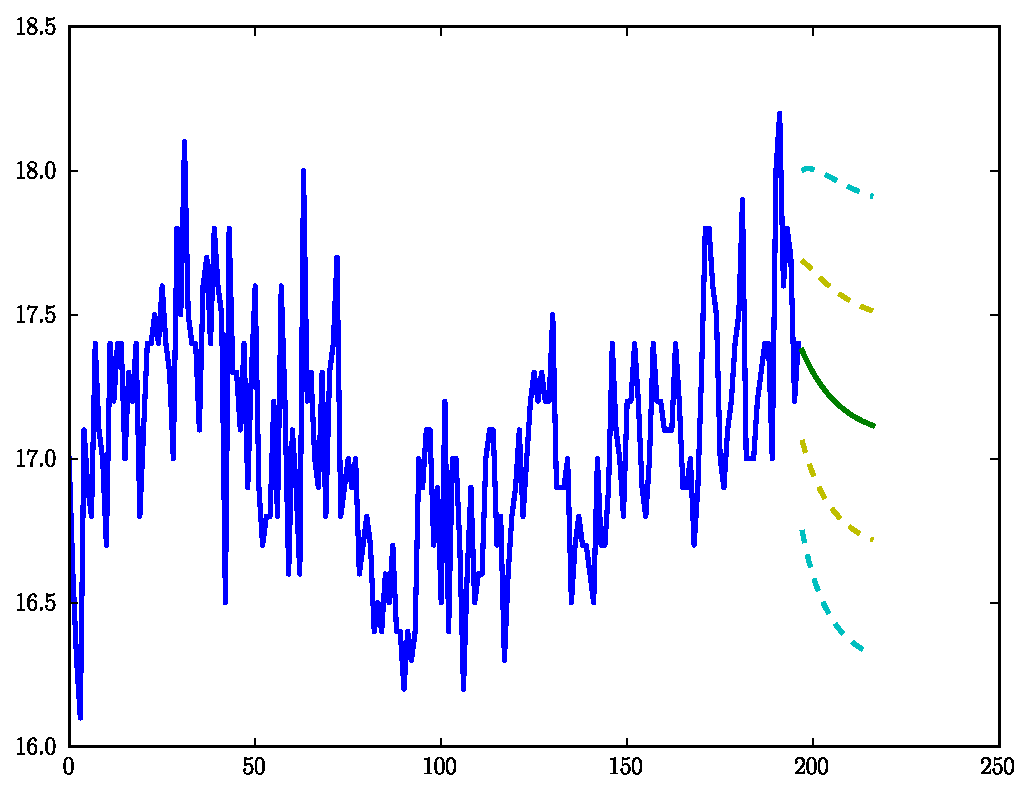
\includegraphics[width=\textwidth]{forecasted_a}
        \end{subfigure}%

        \begin{subfigure}[b]{0.7\textwidth}
                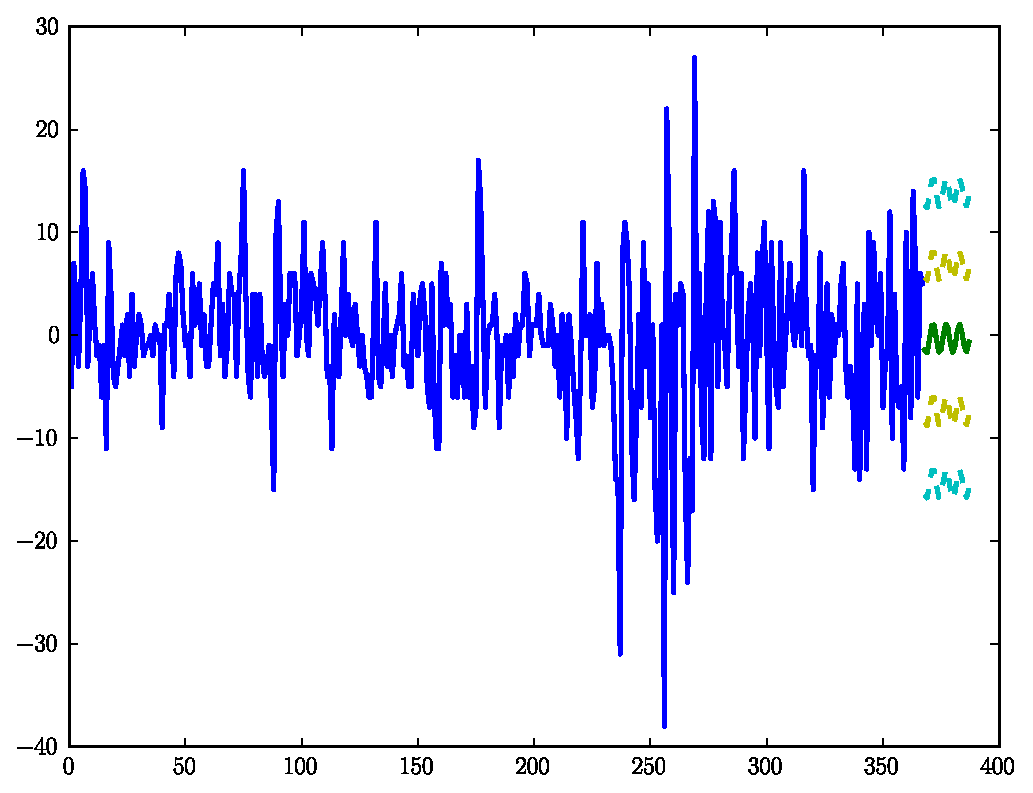
\includegraphics[width=\textwidth]{forecasted_b}
        \end{subfigure}

        \begin{subfigure}[b]{0.7\textwidth}
                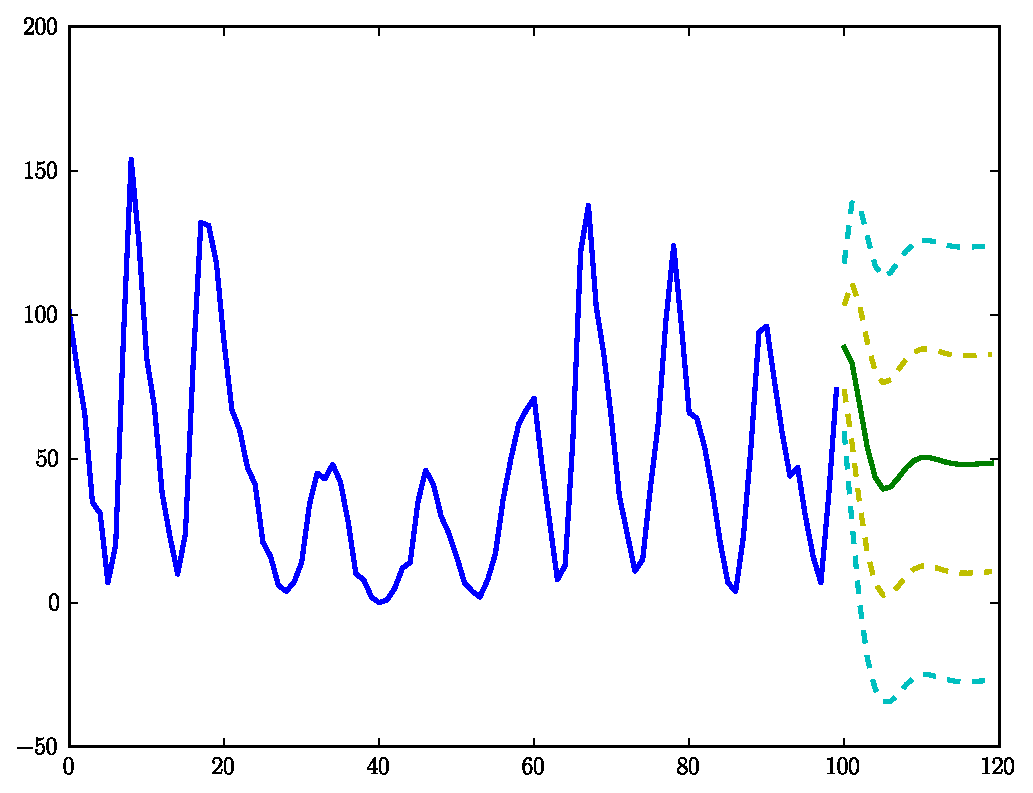
\includegraphics[width=\textwidth]{forecasted_c}
        \end{subfigure}
    \caption{Three time series along with expected value (green), $\pm \sigma_a$ credible interval (yellow),
    and $\pm 2\sigma_a$ credible interval (cyan) of twenty forecasted values.}
	\label{fig:forecasted}
\end{figure}

\begin{comment}

The Box-Jenkins methodology may be too esoteric, in light of straightforward
alternatives such as the AICc. I have decided to leave this material out.

\section*{Identification}

If we have a time series $\{z_t\}$ and wish to fit an $ARMA(p,q)$ to it, we
must first identify the order of the model, that is, what $p$ and $q$ should
be. We discuss a methodology presented by Box and Jenkins that depends on the
autocorrelations and partial-autocorrelations of the data. Alternative methods
exist, such as using the Akaike information criterion with a correction (AICc).

\subsection*{Autocorrelation}

The autocorrelation between between $z_{t}, z_{t+k}$ is defined as the
normalized covariance between the two random variables, verbosely given as
\begin{align}
    \label{eq:arma:autocorrelation}
    \text{cor}[z_{t}, z_{t+k}] = \frac{E[(z_{t} - E[z_{t}])(z_{t+k} -
    E[z_{t+k}])]}{\sqrt{E[(z_{t} - E[z_{t}])^2(z_{t+k} - E[z_{t+k}])^2]}}
\end{align}
Since the $\{z_t\}$ is assumed to be covariance-stationary,
\ref{eq:arma:autocorrelation} depends only on the lag $k$, not on $t$. This
justifies the notation
\begin{align}
    \rho_k = \text{cor}[z_{t}, z_{t+k}] \quad \forall t
\end{align}
When $\rho_k$ is considered a function of $k$, it is called the autocorrelation
function. Since $\rho_0 = 1, \rho_{-k} = \rho_k$, we will be interested in the
cases when $k > 0$. We can estimate $\rho_k$ from sample data as
\begin{align}
    \label{eq:arma:autocorrelation_estimate}
    \hat{\rho}_k = \frac{\sum_{t=1}^{N-k}(z_t - \hat{\mu})(z_{t+k} -
    \hat{\mu})}{\sum_{t=1}^{N}(z_t - \hat{\mu})^2}
\end{align}
where $\hat{\mu}$ is the sample mean. This is one of a number of estimates of
autocorrelation.

\begin{problem}
\label{prob:arma:autocorrelation}
Write a function that computes the autocorrelation estimate described in
\ref{eq:arma:autocorrelation_estimate}, given a time series and a lag $k$.
Plot $\hat{\rho}_k$ for $1 \leq k \leq 20$ for each of the three data sets.
\end{problem}

\subsection*{Partial-Autocorrelation}

\end{comment}
